\section{Experimental Results}\label{sec:results}

\subsection{Experimental Setup}\label{sec:xp_setup}
%
\begin{figure}[ht!] %FIXME: this figure is not referenced.
  \begin{center}
    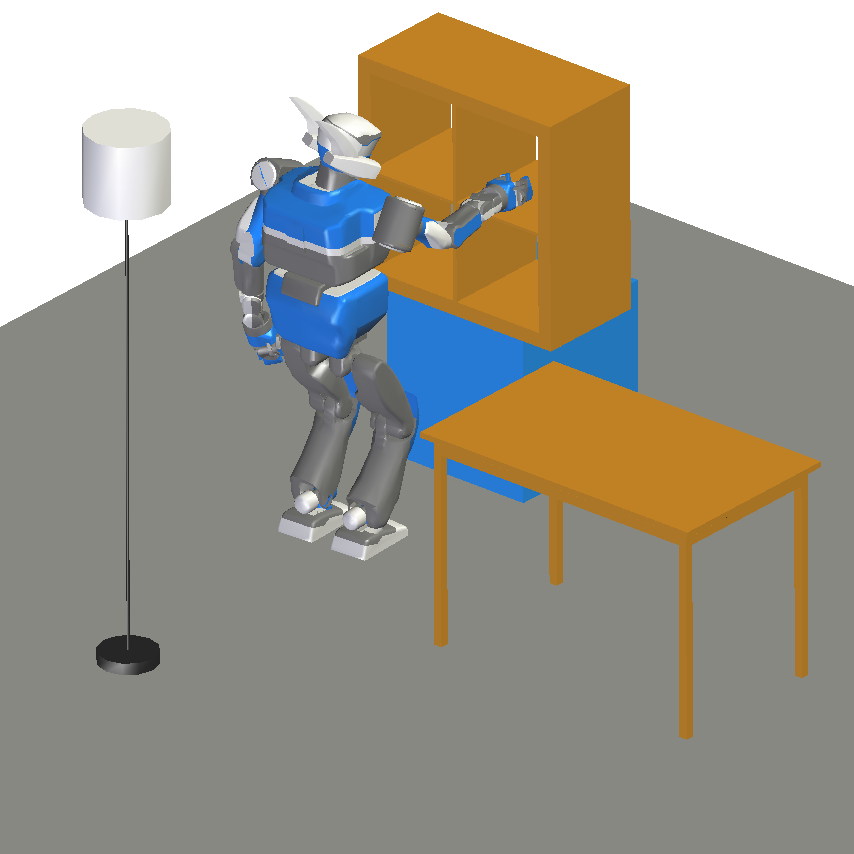
\includegraphics[width=\linewidth]{images/trajectory-8.png}
  \end{center}
  \caption{The HRP-2 robot drops a ball on a shelf while localizing
    itself using vision based localization. \label{fig:xp_setup_screenshot}}
\end{figure}
%
The experiment demonstrates that by localizing the robot while walking, HRP-2 can reach a goal position independently of the
execution errors. In the chosen scenario, the robot must drop a ball on a shelf after walking 2 m. A more precise description of the
scenario is depicted by Fig.~\ref{fig:xp_setup_dim}. Empirically, we estimated the HRP-2 mean drift to be around one cm per
step. Considering that 32 steps are required to reach the goal without hitting the obstacles, the usual drift would prevent the task from
being accomplished.
%
\begin{figure}[ht!]
  \begin{center}
    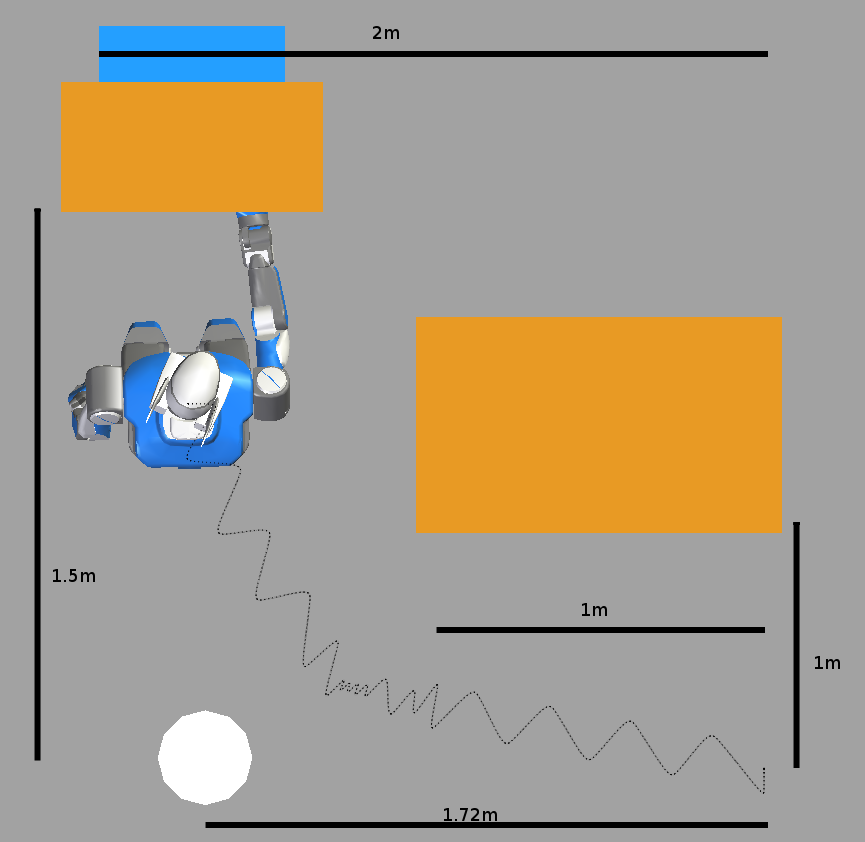
\includegraphics[width=\linewidth]{images/dimensions.png}
  \end{center}
  \caption{Experimental setup description (top view). The dotted line displays the robot waist trajectory.\label{fig:xp_setup_dim}}
\end{figure}
%
The camera trajectory estimated by the localization algorithm is validated using motion capture data. Markers have been placed on both the robot head and left ankle to provide ground truth.

Finally, the camera position is given by the algorithm described in detail in the previous sections. The localization module has been running at a mean rate of 16\hertz~during the experiments. The vision computer running the vision based localization node is a Intel\textregistered Core\texttrademark\ 2 CPU T7200~@~2.00GHz with 2Gb.\ of RAM.

During the experiments, the robot sometimes failed to drop the ball properly. It was either due to a bad initialization which sometimes lead to localization failure or to robot flexibility. Indeed, the shelves is quite narrow and the robot ankles passive joints were generating hands movements which were causing collisions, even though the robot localization is precise enough. It would be interesting in a
future work to not only localize the robot with respect to an absolute frame but also switch to a task-based localization at the end to correct the hand trajectory and avoid collisions.

On our platform, the vision localization module returned a pose at around 16~\hertz. On the opposite, the HRP-2 robot uses a control loop
at 200~\hertz. To preserve real-time, the real-time component was communicating the robot configuration asynchronously at around
75~\hertz. The error estimation components was running at a mean rate of 10~\hertz. As a correction is added every two steps, it was not
useful to evaluate the error at a higher frequency.

\subsection{Comparison to Motion Capture Data}\label{sec:mocap}

Fig.~\ref{tab:mocap_comparison} contains the camera position estimated by the motion capture system and by the localization algorithm. The
mean error is 0.2 m in translation. Drop in the algorithm precision can occur when the robot enters a part of the map which is not dense
enough or where the environment does not incorporate enough texture to detect enough interest points. It happens in our scenario near the end when the camera is too close to the shelf to perceive its environment correctly.

The used motion capture system is a Motion Analysis system relying on six Eagles and four Hawks cameras. It provides an estimation of the
camera position at 200~\hertz~with a precision error of less than one cm.
%
\begin{figure}[ht!]
  \begin{center}
    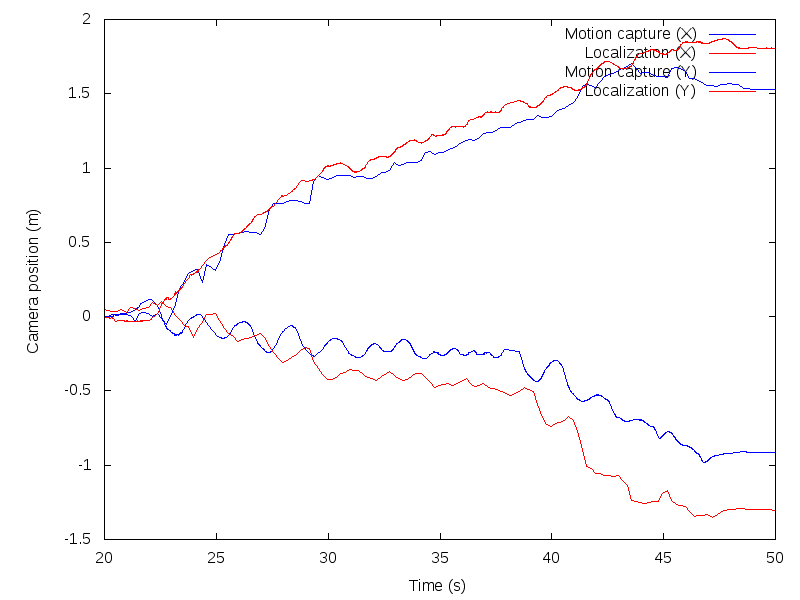
\includegraphics[width=\linewidth]{data/mocap.png}
  \end{center}
  \caption{Camera position estimated by both the motion capture system
    and the localization algorithm. \label{tab:mocap_comparison}}
\end{figure}
%

%%% Local Variables:
%%% ispell-local-dictionary: "american"
%%% LocalWords:  odometry HRPs
%%% End:
